\documentclass[11pt]{article}

\pdfminorversion=4

% use packages
\usepackage[utf8]{inputenc}
\usepackage{amsmath}
\usepackage{amsthm}
\usepackage{amsfonts}
\usepackage{amscd}
\usepackage{amssymb}
\usepackage{natbib}
\usepackage{url}
\usepackage[table,xcdraw,usenames]{xcolor}
%\usepackage[usenames]{color}

% \usepackage[pdftex,active,tightpage]{preview}
% \setlength\PreviewBorder{2mm}

\usepackage{tikz}

% \usetikzlibrary{arrows,positioning, calc}
% \tikzstyle{vertex}=[draw,fill=black!15,circle,minimum size=20pt,inner sep=0pt]

\usetikzlibrary{trees}

% \usepackage{tikz-qtree,showframe}

\usepackage{forest}


\usepackage{graphicx}
\usepackage{subcaption}
\usepackage{mathtools}
\usepackage{enumitem}
\usepackage{authblk}
\usepackage{bm}
\usepackage{comment}
\usepackage{pdfpages}

\usepackage{hyperref}
\usepackage{caption}
\usepackage{float}
%\usepackage[caption = false]{subfig}
\usepackage{tikz}
\usepackage{multirow}
\usepackage[linesnumbered, ruled,vlined]{algorithm2e}
\usepackage{pdflscape}
\usepackage{etoolbox}

%\AtBeginEnvironment{align}{\setcounter{equation}{0}} % https://tex.stackexchange.com/questions/349247/how-do-i-reset-the-counter-in-align

% margin setup
\usepackage{geometry}
\geometry{margin=0.8in}

% function definition
\newcommand{\V}{\textbf{V}}
\newcommand{\weight}{\pi}
\newcommand{\ret}{\textbf{r}}
\newcommand{\y}{\textbf{y}}
\newcommand{\w}{\textbf{w}}
\newcommand{\x}{\textbf{x}}
\newcommand{\dbf}{\textbf{d}}
\newcommand{\X}{\textbf{X}}
\newcommand{\Y}{\textbf{Y}}
%\newcommand{\L}{\textbf{L}}
\newcommand{\Hist}{\mathcal{H}}
\newcommand{\Prob}{\mathbb{P}}
\def\mbf#1{\mathbf{#1}} % bold but not italic
\def\ind#1{\mathrm{1}(#1)} % indicator function
\newcommand{\simiid}{\stackrel{iid}{\sim}} %[] IID 
\def\where{\text{ where }} % where
\newcommand{\indep}{\perp \!\!\! \perp } % independent symbols
\def\cov#1#2{\mathrm{Cov}(#1, #2)} % covariance 
\def\mrm#1{\mathrm{#1}} % remove math
\newcommand{\reals}{\mathbb{R}} % Real number symbol
\def\t#1{\tilde{#1}} % tilde
\def\normal#1#2{\mathcal{N}(#1,#2)} % normal
\def\mbi#1{\boldsymbol{#1}} % Bold and italic (math bold italic)
\def\v#1{\mbi{#1}} % Vector notation
\def\mc#1{\mathcal{#1}} % mathical
\DeclareMathOperator*{\argmax}{arg\,max} % arg max
\DeclareMathOperator*{\argmin}{arg\,min} % arg min
\def\E{\mathbb{E}} % Expectation symbol
\def\mc#1{\mathcal{#1}}
\def\var#1{\mathrm{Var}(#1)} % Variance symbol
\def\checkmark{\tikz\fill[scale=0.4](0,.35) -- (.25,0) -- (1,.7) -- (.25,.15) -- cycle;} % checkmark
\newcommand\red[1]{{\color{red}#1}}
\def\bs#1{\boldsymbol{#1}}
\def\P{\mathbb{P}}
\def\var{\mathbf{Var}}
\def\naturals{\mathbb{N}}
\def\cp{\overset{p}{\to}}
\def\clt{\overset{\mathcal{L}^2}{\to}}

\setcounter{tocdepth}{4}
\setcounter{secnumdepth}{4}

\newtheorem{corollary}{Corollary}
\newcommand{\ceil}[1]{\lceil #1 \rceil}
\newcommand{\norm}[1]{\left\lVert#1\right\rVert} % A norm with 1 argument
\DeclareMathOperator{\Var}{Var} % Variance symbol

\newtheorem{cor}{Corollary}
\newtheorem{lem}{Lemma}
\newtheorem{thm}{Theorem}
\newtheorem{defn}{Definition}
\newtheorem{prop}{Proposition}
\theoremstyle{definition}
\newtheorem{remark}{Remark}
\hypersetup{
  linkcolor  = blue,
  citecolor  = blue,
  urlcolor   = blue,
  colorlinks = true,
} % color setup

% proof to proposition 
\newenvironment{proof-of-proposition}[1][{}]{\noindent{\bf
    Proof of Proposition {#1}}
  \hspace*{.5em}}{\qed\bigskip\\}
% general proof of corollary
  \newenvironment{proof-of-corollary}[1][{}]{\noindent{\bf
    Proof of Corollary {#1}}
  \hspace*{.5em}}{\qed\bigskip\\}
% general proof of lemma
  \newenvironment{proof-of-lemma}[1][{}]{\noindent{\bf
    Proof of Lemma {#1}}
  \hspace*{.5em}}{\qed\bigskip\\}

\allowdisplaybreaks

\title{Forecast Adjustment Under Shocks: A Unification}
\author{David P. Lundquist\thanks{davidl11@ilinois.edu}, Daniel J. Eck\thanks{dje13@illinois.edu} }
\affil{Department of Statistics, University of Illinois at Urbana-Champaign}
\date{\today}

\begin{document}

\maketitle

\begin{abstract} 
  When should one's default forecasting model be adjusted, augmented, or abandoned completely?  Should it be done algorithmically or via human discretion, and if the latter, how much discretion?  Should an adjustment be carried out using external information, and what exactly should be adjusted?  This work systematizes and unifies the rich landscape of model adjustment and model correction methods, with a special focus on forecast adjustment under the presence of news shocks, when unanticipated events may give an observer reason to doubt the credibility of the default forecasting function.  We demonstrate the usefulness of similarity-based methods in forecasting and present a general framework dubbed Similarity-based Parameter Correction (SPC).  We highlight several specific time series models that can benefit from SPC, along with formal results for some of those special cases.
\end{abstract}


\section{Introduction}\label{Introduction}

For various modeling and prediction tasks in time series and panel data, the salient challenge is not predicting when an event will occur but what its key properties will be.  In the familiar case of scalar time series, those properties can include the time series' post-event direction, magnitude of change, moments, duration of the event, and correlation structure, all over an arbitrary horizon or perhaps multiple horizons. This is not to say that predicting the arrival of an event is easy. In some cases, it may be difficult or impossible, and the event might not even be conceivable to many before it happens, as was the case with the COVID-19 pandemic.  There, reacting sensibly to a shock or structural change may best one can hope for. 

Herein we attempt to unify a range of conceptual approaches to forecasting amid shocks that have developed across the broad ecosystem of the econometric and forecasting literatures.  We attempt to locate our main contribution, Similarity-based Parameter Correction, at the intersection of several important strands of thought.  Additionally, we delineate a specific type of SPC called post-shock forecasting, which is induced by nuanced and interesting choices that fall under the general SPC framework.  In particular, this work focuses on model adjustment amid news shocks that undermine the reliability of the  model at hand.  Forecasting under shocks raises unavoidable questions: should the forecast model be abandoned in favor of a discretionary or ad-hoc or one-off adjustment?  Does the does the discretion of a forecaster rule out a quantitative method for making the adjustment?  What is the ultimate purpose of the adjustment, and how it is to be used?  For how long is the adjustment necessary or reliable?

Forecast model adjustment, known most widely perhaps by the term intercept-correction, has received the most attention in several articles and book chapters \citep{hendry1994theory,clements1996intercept,clements1998forecasting}.  Of special importance is the distinction between discretionary and automated intercepts corrections. \cite{hendry1994theory} define scalar intercept corrections to be automated when they follow the simple rule of adding an estimation or prediction residual $e_{t}$ to subsequent (possibly but not necessarily all) forecasts $\hat f_{t+1},\hat f_{t+2},[...].$.  ``\textit{[S]etting the model back on track}" is the informal label they provide for that procedure.  It must be noted here that adding a past residual to future forecasts assumes implicitly that whatever caused the residual is persistent, and hence intercept correction makes more sense for levels.  That is, of course, unless one has a sense of how long the intercept correction will be needed for.
 
In \cite{hendry1994theory}, after recounting the bipartite division of interception corrections in discretionary and automated varieties, the authors present a six-way taxonomy of information that a modeler possesses at the time a forecast is made.  The authors also consider structural change in the data-generating process during the forecast period, including as early as the first point in the forecast period (specifically in the autoregressive structure), as well as what is for them the more interesting case: structural change between $T^{*}-1$ and $T^{*}$.  This current work finds both cases interesting.  The term intercept correction itself can be both a bit deceptive in limiting, in that it need not pertain to intercepts.  \cite{hendry1994theory} themselves note the possibility of correcting a coefficient in a forecast model specification, and \cite{guerron2017macroeconomic} developed a similarity-based procedure for correcting $\beta$ using past information of the time series itself.   For a review of more recent work in similarity-based forecasting, we refer the reader to \cite{lundquist2024volatility}.

What if the break in the DGP is brought about by a very particular kind of event, a news shock?   What if we could predict well the intercept shift that occurs between $T^{*}$ and $T^{*}+1$?  In \cite{castle2016overview}, the authors list six necessary conditions for reacting to what we in this current paper call a news shock.  Of greatest interest to us are two of the six: ``the forecasting model already embodies that source of information" and ``there is an operational method for selecting
an appropriate model".   For such cases, forecasting procedures have been explored in \cite{lin2021minimizing,lundquist2024volatility}, where the AR(1) and GARCH($m,s$) cases, respectively, are treated.  Both works target additive parameters in scalar time series, predicting those random effects by aggegating information from other time series.  The authors leave several stones unturned, including a more general, dare say comprehensive treatment of how to forecast under any sort of shock.

As the literature has developed, a current practitioner of forecast adjustment can now choose between (i) procedures that are discretionary or automated, (ii) whether the data is internal (i.e. from the time series itself) or external, (iii) the term to be corrected (e.g. intercept, coefficients), if any, (iv) as well as the correction function (i.e. the mapping from the donor unit data to the correction term in the time series under study), including the weighting applied to the assembled data (e.g. Nearest-Neighbor, arithmetic mean, kernel methods).  We discuss this in depth in Section \ref{global_overview}.

The procedure presented, post-shock forecasting, is a discretionary procedure for intercept correction that integrates data internal or external to the time series under study in a systematic manner.  The correction function uses the notion of similarity between breaks in different time series, it and borrows from the causal inference literature to aggregate information from those similar circumstances.  Beyond of \citet{lin2021minimizing,lundquist2024volatility}, we are not aware of prior work uses a parametric specification for nonzero errors as well as a method for aggregating similar shocks occurring outside the time series under study.

The structure of this manuscript is as follows.  We first provide a review of several disparate time series literatures, including intercept correction, model-evaluation, and similarity-based forecasting.  We then provide a canonical setting in which we attempt to focus our work.  This setting will be presented at a level of generality that showcases the broad applicability of our method.  We then introduce the method from a global perspective, abstracting away from familiar applications.  We then show several specific applications, including novel applications that cannot be found elsewhere in the literature.  We close with a discussion, including possible extensions.

\subsection{History of and Motivation for Intercept Correction\label{intercept_correction}}

Intercept correction is the correction of a forecast by adding the residual at time $t$ to the forecasts at some subset of $\{t+1,t+2,...\}$.  We are doing something very close to that which is adding the predicted correction function output at time $t$ to the forecasts at some subset of $\{T_{1}^{*}+1,T_{1}^{*}+2,...\}$, where $T^{*}_{1}$ is the shock time of the time series under study. 
  \cite[p. 177]{hendry1994theory} note that a break in the DGP (and hence the misspecification of the default forecasting method) is the ``most obvious and best understood rationale'' for intercept correction.  To be sure, this manuscript will make its contributions largely in this area.  However, before we get there, let's follow Clements, Hendry and other authors in asking whether we would ever want to intercept-correct an unconditional forecast as opposed to the conditional.  This is what Clements and Hendry call ``Exploiting the information in unconditional forecasts''.  \cite[p. 170-1]{hendry1994theory} recall how unconditional forecasts can have lower forecast variance than conditional forecasts.  There seems to be two different questions that we should distinguish: we forecast would minimize the conditional expectation of MSE, and what forecast would have the lowest variance.

  Mismeasured data is discussed in \cite[p. 166]{hendry1994theory} as a motivator for intercept correction.  Could similarity-based correction help?  Here is an idea: if we believe that our most recent measurement of the series is noisy, we can disregard the point itself and instead take a convex combination of that point and the \cite{lin2021minimizing}-style prediction based on aggregation.

 Yet another potential motivation springs from the way we evaluate model performance.
Evaluating a Model by Forecast Performance \cite{clements2005evaluating}
\begin{enumerate}
  \item   unconditional versus conditional, models;
  \item internal versus external standards;
  \item checking constancy versus adventitious significance;
  \item ex ante versus ex post evaluation (skip this one?);
  \item 1-step versus multi-horizon forecasts -- this is a relevant question to ask in the context of post-shocking forecasting: should we correct the earliest forecast and then allow the shock to propagate, or should we just correct each term in the horizon, h=1, 2,..., H?
  \item in-sample fixed coefficients versus continuous updating
\end{enumerate}

Here is one argument: if we are going to judge a model by forecast performance, we need to entertain the possibility that the model may breakdown and that our pre-breakdown-based criteria for model performance will be invalidated. \textcolor{red}{Here is how that matters for this paper: if you have a family of models estimated used a Gaussian loss function, and the post-shock residuals are not conditionally Gaussian (e.g. they could be conditionally Cauchy), then why even start with the default forecasting function?  Why not throw it out entirely?  If only the distribution of the innovations changes, then would that even matter for a forecast that is purely concerned with the conditional mean?}

\subsection{Forecasting Amid Shocks}

In this section, we wish to locate the task of forecasting amid shocks within the broader literature on forecasting under breaks in the GDP.  \cite{castle2011forecasting} discusses necessary conditions for forecasting under breaks as well as a taxonomy of information available for doing so.  They also make a fundamental distinction between ``regular forces'' and alternative sources of information for making forecasts.  Most interesting, their discussion of ``forecasting facing a shift in the intercept of a model of a variable y induced by another observable variable z" represents the most similar idea to  \cite{lin2021minimizing,lundquist2024volatility} --- with one important disclaimer.  In those later two works, the variable $z$ is observable and yet not quantitative.

In \cite{clements2005guest} (cited in \cite{castle2013forecasting}), the authors note that when forecasts fail, it often has to do with location (i.e. intercept shifts), and therefore using additional information is not likely to help unless it can address potential location shifts.  \cite{rossi2021forecasting} says that breaks in a model's parameters are not necessary or sufficient to generate time variation in forecasting performance.  

\cite{hendry2004pooling} discuss that intercept correction can improve forecasts under structural breaks as well as under ``deterministic misspecification'', by which they mean misspecification not caused by stochastic events like location shifts.  The same two justifications exist for SPC: we can use SPC when we know there to be a structural break, and we can also use it when we know our model is wrong and want to correct a parameter for some critical forecasting task.

\subsection{Forecasting Using Outside Information}\label{outside_info}

When is more information better?  That is a central question with regard to forecasting.  For example, admidst a shock, should we avail ourselves of additional internal information or external information?\\

Incorporation of Outside Information is the Norm, Not the Exception. \\ 

Are there cases where it is ambiguous whether information should count as internal or external to the time series under study?

ARMA models and other models that model the future as a function of only the past values and past innovations of the series itself are well-known to be unrealistic as a data-generating processes.  They are also well-known to be poor predictors of the future.  What we are doing here is therefore not out of the ordinary but distinct in at least two ways: (1) we are incorporating outside information faster, and (2) we are proposing a principled, systematic way to do it that defies that curse of dimensionality.  If one wanted to forecast using linear models and high-dimensional information set, then some kind of method for reducing model complexity would be required.  We avoid that.

\textcolor{red}{The draft here transitions to similarity, since the manuscript under development is at the intersection of post-break forecasting and similarity-based forecasting.  In particular, it uses the former to motivate the latter.}
Now we discuss The Meaning and Use of Similarity
Hume? Cite Israeli authors, if so.  The notion of similarity appears in various statistical contexts, including matching, synthetic control, nearest-neighbor methods, not to mention the massive area of approximation theory.  The uses of similarity are too sprawling to recount in detail.  Below we talk about how it could matter in this work.

Similar, in the strong sense, could mean that a shared DGP exists. It could mean similar in the covariates that parameterize the shocks.  It matters where we look for similarity and how we estimate similarity.

Quantitative ways of determining similarity include matching a target object to other objects along one or more variables, where exact matches may be likely or may be statistically impossible.  In metric spaces, the notion of a metric that quantifies nearness is crucial to fundamental concepts of proximity.  This suggests an optimization problem such that, for any target object $Q$, the search for similarity means a search for an approximator $A$ s.t. $\delta(Q,A)$ is smallest, where $\delta$ is an appropriate metric.

Asymmetric distance functions (which are of course not metrics) are useful when we want to explore differences between donors and weight different contributors to that function differently.  Consider an asymmetric Jaccard Index $\delta_{\mathcal{J}}(\cdot,\cdot)$ that is maps from any two finite-cardinality sets to the interval $[0,1]$ \citep{garg2015asymmetric}.  So far, we have discussed only binary measures of similarity.  The distance-based weighting scheme found in \cite{lin2021minimizing} and repurposed in \cite{lundquist2024volatility} can be thought of as an $n$-ary similarity measure, where the $n$ weights means little in isolation but can tell a greater story when viewed alongside the approximation they produce.

What about qualitative ways of determining similarity?  In \cite{lundquist2024volatility}, donors are identified by matching the qualitative aspects of the shock in the time series under study to shocks previously witnessed in other series.  Only after the donor pool has been identified based on qualitative facts about the shocks is there a role for quantative tools. 

% \begin{preview}
% \begin{tikzpicture}[very thick,level/.style={sibling distance=180 mm/#1}]
% \node [vertex] (r){Forecast Model Adjustment}
%   child {
%     node [vertex] (a) {Break in the GDP at $T^{*}$}
%     child {
%       node [vertex] {$20$}
%       child {
%         node [vertex] {$-3$}
%         child {node [vertex] {$17$}}
%         child {node [vertex] {$5$}}
%       }
%       child {node [vertex] {$6$}}
%     }
%     child {
%       node [vertex] {$3$}
%       child {node [vertex] {$7$}}
%       child {node [vertex] {$2$}}
%     }
%   }
%   child {
%     node [vertex] {Break in the GDP at $T^{*}$}
%     child {
%       node [vertex] {$8$}
%       child {node [vertex] {$2$}}
%     }
%     child {
%       node [vertex] {$11$}
%       child {node [vertex] {$17$}}
%       child {node [vertex] {$-4$}}
%     }
%   };
% \end{tikzpicture}
% \end{preview}


% https://tex.stackexchange.com/questions/64148/tikz-label-on-tree-edge

% \begin{forest}
% for tree={circle,draw, l sep=20pt}
% [3,red 
%     [1  
%       [4,edge label={node[midway,left] {Help!}} ] 
%       [1] 
%       [3]
%     ]
%     [2
%       [3] 
%       [2] 
%       [5]
%   ] 
% ]
% \end{forest}


%https://tex.stackexchange.com/questions/64148/tikz-label-on-tree-edge

%  \begin{tikzpicture}[level distance=1.5cm,
%   level 1/.style={sibling distance=3.5cm},
%   level 2/.style={sibling distance=2.5cm}]
%   \tikzstyle{every node}=[circle,draw]
  
% \node (Root) [red] {Is there a break in the DGP between T* and T*+1?} 
%     child {  edge from parent node[left,draw=none] {Do you have information outside of the “regular forces”
%     } 
%     node {Yes} 
%     child { node {Yes} 
%             child { node{Yes} edge from parent node[left,draw=none] {lab} }
%             child { node{No}}}
%     child { node {No} }
% }
% child { 
%     node {No}
%     child { node {Yes} }
%     child { node {No} }
% };
% \end{tikzpicture}

% \noindent\begin{forest}
%   for tree={
%     parent anchor=south,
%     child anchor=north,
%     edge path={
%       \noexpand\path [\forestoption{edge}] (!u.parent anchor) -- +(0,-5pt) -| (.child anchor)\forestoption{edge label};
%     }
%   }
%   [Is there a break in the DGP between T* and T*+1?
%     [Extractive Summarization
%       [Similarity
%         [Topic]
%         [Cluster]
%       ]
%       [Classification
%         [test2]
%         [test1]
%       ]
%       [Feature Selection
%         [test1]
%         [test2]
%         [test3]
%       ]
%       [Feature Extraction
%         [test2]
%         [test3]
%       ]
%     ]
%     [Abstractive Summarization]
%   ]
% \end{forest}
% \bigskip

% https://tex.stackexchange.com/questions/539600/tikz-forest-coloring-and-edge-label-positions

% \tikzset{eln/.style={midway, font = \scriptsize,circle,inner sep=2pt}}
% \begin{forest}
% for tree = {circle, 
%     draw=red, %<-added =red
%     minimum width = 2.25em,
%     l sep+=2em
% }
%     [\textcolor{blue}{Is there a break in the DGP between T* and T*+1?
% }
%         [Dog, edge label = {node [above left,eln] {\textcolor{green}{Yes}}}
%             [$B$, edge label = {node [above left,eln] {$4$}}
%                 [$D_1$, edge label = {node [left,eln] {$7$}}
%                     [$G_1$, edge label = {node [left,eln] {$10$}}]
%                 ]
%             ]
%             [$C$, edge label = {node [above right,eln] {$2$}},edge=blue%<-blue edge
%                 [$D_2$, edge label = {node [above left,eln] {$3$}}
%                     [$G_2$, edge label = {node [left,eln] {$6$}}]
%                 ]
%                 [$G_3$, edge label = {node [above right,eln] {$4$}}]
%             ]
%         ]
%         [$G_4$, edge label = {node [above right,eln] {\textcolor{red}{No}}}]
%    ]
% \end{forest}

%https://tex.stackexchange.com/questions/226435/reducing-forest-tree-width-without-squashing


%https://tex.stackexchange.com/questions/244006/making-forest-tree-with-lots-of-text-much-narrower
\begin{figure} 
  \centering  
\resizebox{\textwidth}{!}{%
\begin{forest}
  /tikz/every node/.append style={font=\small},
  for tree={
    rounded corners, 
    % top color=gray!5, bottom color=gray!30, 
    edge+={darkgray, line width=4pt}, 
    draw=darkgray, 
    l sep=.8cm,
    s sep=.5cm,
    minimum height=8.8cm,
    minimum width=1cm,
    child anchor=west,
    parent anchor=east,
    grow'=east,
  minimum size=1cm,%new possibility
  text width=4cm,%
    draw,
    anchor=west,
    edge path={
      \noexpand\path[\forestoption{edge}]
        (.child anchor) -| +(-5pt,0) -- +(-5pt,0) |-
        (!u.parent anchor)\forestoption{edge label};
    },
  }
    [Break in the DGP between $T^{*}$ and $T^{*}+1$?,fill=blue!30 
        [Is there information outside of “regular forces” \citep{castle2011forecasting},edge=green, fill=blue!30%,draw=green
            [Can we use the information outside “regular forces” to forecast (as opposed to merely spotting the break)?,edge=green,,fill=blue!30 
                [Do you have a parametric model (with estimable parameters) for how information outside of ``regular forces” will figure at $T^{*}+h$?,edge=green,fill=blue!30 
                  [What other time series are governed by the parametric model?  How can we extract information from them?  Which are most relevant, %most similar?  How do we determine similarity, quant or qual?  Once we know what is similar, how do we use it?
                  ,edge=green,fill=blue!30 
                  ]
                  [The information that helped spot the break can be used to assemble series that have experienced breaks under similar circumstances. Forecast residuals/losses can be aggregated. %basement for model adjustment for the time series under study.  Without a parametric model, your options are limited but not empty.  With appropriate assumptions on the DGP pre-break and post-break, assumptions on the forecast functions and misses, we can still do things like aggregate residuals and bound forecast loss.
                  ,edge=red,fill=gray!30
                  ]
                  ]
                [Use “regular forces” to do the model adjustment for the post-break period.  Examples of this would include refitting one’s data to use Markov-switching models – i.e. using only the series itself.,edge=red,fill=gray!30
                ]
                ]
                [Then forecasting will require at least one post-break data point to be observed.,edge=red,fill=gray!30]
            ]
            [\cite{clements1998forecasting} discuss this.,edge=red,fill=gray!30]
            ]
        ]
    ]
\end{forest}
}\caption{Forecast Model Adjustment: A Decision Tree}\label{fig:tree}
\end{figure}


\section{Setting}\label{Setting}

In order to introduce the general framework for adjusting forecasts under shocks, we provide an illustration.  In Figure \ref{fig:motivating_piece_convex_combination}, we borrow from \cite{lundquist2024volatility} to show how the aggregation of estimated excess volatilities from donors in the donor pool works when the correction function is a specially-chosen convex combination of fixed effects from the donor pool.  

In this work, we will be focused on shocks that occur strictly between two discrete time points, or informational available at a ``fractional lag" \citep{castle2011forecasting}.  This raises an important terminological point.  Errors are a staple of stochastic modeling, and certainly no proper inventory of the wide range of uses of ``noise", ``shocks", and so can be accomplished here.  Whereas in the psychometric and social-scientific fields, errors may represent unmeasured or latent capacities of a unit, in other fields like the natural sciences, errors may be used to account for variability in the instruments used to collect data.  ``Innovations" or ``shocks", in econometric literature, are generally understood to represent the arrival of previously unknown (but not necessarily uncontemplated) information.  Shocks are called structural when they are can be linked back to some key feature of an scientific (usually economic) theory; otherwise, they are idiosyncratic.  However, there exist other subcategories of shocks that crosscut the distinction just made.  For example, a news shock is a shock in which the information material to the market is delivered via newsmedia and moves markets no earlier than the news.  Shocks can also be permanent or transitory, supply-related or demand-related, and so forth.  The taxonomy is vast.  What matters for this work is the news shocks we posit occur between two discrete time points, so that a practitioner is faced with the question of what action is most advisable for the following time point, given the news shock.

\subsection{Formal Modeling Setup}

  \begin{figure}[h!]
    \begin{center}
      \begin{tikzpicture}
        \node[anchor=south west,inner sep=0] at (0,0) {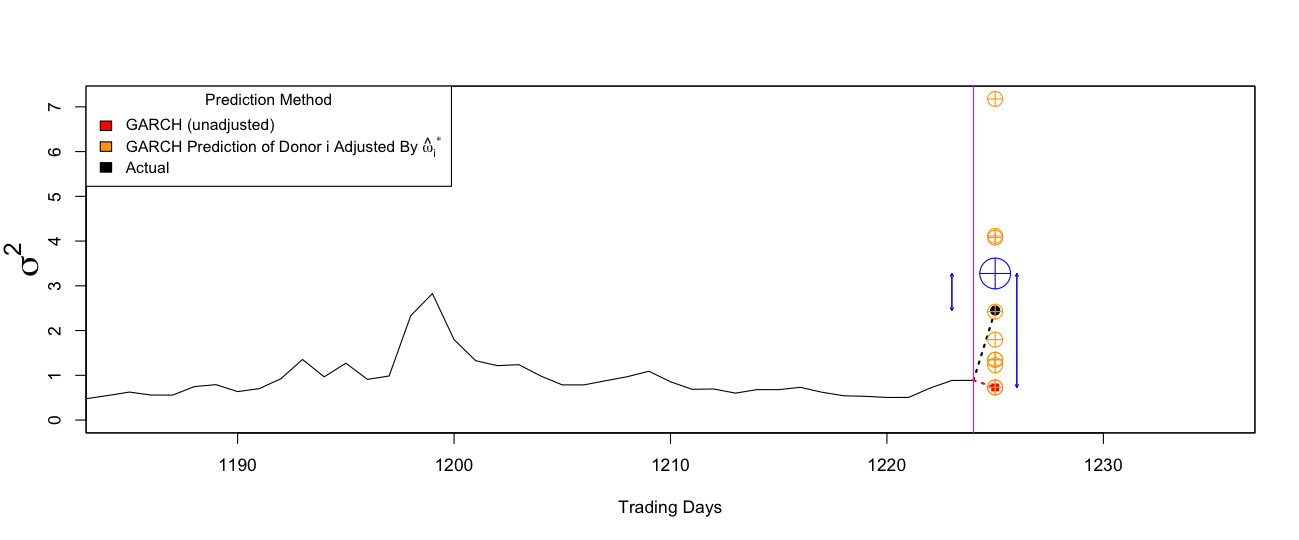
\includegraphics[width=\textwidth]{simulation_plots/motivating_piece_convex_combination.png}};
        % \draw[red,ultra thick,rounded corners] (7.5,5.3) rectangle (9.4,6.2);
        % \node[draw,text width=4.45cm] at (9.8,3.2) {$\textcolor{blue}{\hat\sigma^{2}_{adjusted} = \hat\sigma^{2}_{unadjusted} + \hat\omega^{*}}$ };
        % \node[draw,text width=2.62cm] at (14.8,2.8) {$\textcolor{blue}{\hat\omega^{*} = \sum^{n+1}_{i=2}\pi_{i}\hat\omega^{*}_{i}}$ };    
        
    \end{tikzpicture}
      \caption{The simulated time series experiences a volatility shock between trading days 1,656 and 1,657.  The GARCH prediction, in red, fails even to approach the volatility spike at $T^{*}+1$, as do several adjusted predictions, which are orange.  In contrast, the GARCH forecast adjusted by $\hat\omega^{*} = \sum^{n+1}_{i=2}\pi_{i}\hat\omega^{*}_{i} $, a convex combination of the estimated shocks in the donor pool, achieves directional correctness as well as a smaller absolute loss in its prediction.  The pink vertical line serves to indicate the adjustment of size $\hat\omega^{*}$ that allows the blue bullseye to approach more closely the ground truth.}    \label{fig:motivating_piece_convex_combination}
   
      \end{center}
    \end{figure}

We will suppose that a researcher has multivariate time series data $\y_{i,t} = (r_{i,t}$, $\x_{i,t}$), $t = 1,$ $\ldots,  T_i$, $i = 1, \ldots, n+1$, where $r_{i,t}$ is scalar and $\x_{i,t}$ is a vector of covariates such that $\x_{i,t}|\mathcal{F}_{i,t-1}$ is deterministic and observed.  Suppose that the analyst is interested in forecasting $r_{1,t}$, the first time series in the collection, which we will denote \textit{the time series under study}.   We assume the following general data-generating process

\begin{align}
  &y_{i,t} = F(\mathcal{F}_{i,t-1}) + \x^{T}_{i,t}\lambda_{t} + \epsilon_{i,t}\label{core_specification}\\
  &\omega_{i,t}^{*} = D^{vol}_{i,t}[\mu_{\omega^{*}}+\delta^{T}\x_{i,T^{*}_{i}+1}+ u_{i,t}],
\end{align} 
 
\begin{align*}
  \mc{M}_1 \colon \begin{array}{l}
    y_{i,t} = F(\mathcal{F}_{i,t-1}) + \x^{T}_{i,t}\lambda_{t} + \epsilon_{i,t}\\[.2cm]
  \end{array}
  \end{align*}

with time-invariant error structure
  \begin{align*}
    \lambda_{t} &\sim \mc{F}_{\lambda}\text{ with }  \E_{\mathcal{F}_{\lambda}}(\lambda) = \mu_{\lambda_{t}}, \mrm{Var}_{\mc{F}_{\lambda}}(\lambda) = \Sigma_{\lambda_{t}}\\
    \epsilon_{i,t} &\simiid \mc{F}_{\epsilon} \text{ with}  \; \E_{\mc{F}_{\epsilon}}(\epsilon) = 0, \mrm{Var}_{\mc{F}_{\epsilon}}(\epsilon)  = \sigma^{2}_{\epsilon},  \\
    u_{i,t} & \simiid  \mc{F}_{u} \text{ with}  \; \mrm{Var}_{\mc{F}_{u}}(u) = \sigma^2_{u},\\
    \epsilon_{i,t} & \indep u_{i,t}.
    \end{align*}
where $F$ maps objects from the past into future objects of $y_{i,t}$, and $\epsilon_{i,t}$ is mean-zero and uncorrelated across time and donors.  Note that this specification above is capacious enough to include data-generating processes of the form 

\begin{align*} 
  y_{i,t} = \log{Y_{i,t}} = \log{a_{i,t}y_{i,t-k}e^{\x^{T}_{i,t}\lambda_{t}+\epsilon_{i,t}}} = \log{a_{i,t}} + \log{y_{i, t-k}} + \x^{T}_{i,t}\lambda_{t} + \epsilon_{i,t}
\end{align*}
with $k\geq1$ and $a_{i,t}, y_{i,t}$ supported on $\mathbb{R}^{+}$.  The term $\x^{T}_{i,t}\lambda_{t}$ will be deemed the $\textit{correction term}$, and the function

\begin{align*}
  \xi \colon \mathcal{F}_{2,T^{*}_{2}} \times \ldots \times \mathcal{F}_{n+1, T^{*}_{n+1}} &\to \mathcal{F}_{1,T^{*}_{1}+h}\\
\end{align*}
that estimates or predicts $\x^{T}_{1,T^{*}+h}\lambda_{T^{*}+h}$ will be deemed the \textit{correction function}.  The correction function maps observable, deterministic events and unobservable events into a space so that something might be learned about $\lambda_{t}$.  If $\x_{i,t}$ were not observable or not deterministic with respect to $\mathcal{F}_{t-1}$, then the correction term would represent an additional error term (not necessarily idiosyncratic).

We require that each time series $\y_{i,t}$ is subject to an observed news event following $T^*_i \leq T_{i} + 1$ and before witnessing $T^*_i+1$.  The reasons for this represent the heart and soul of the framework proposed.  We are not proposing a method to correct for unanticipated shocks that have been reflected in the observed data.  Instead, we are proposing a method to correct for shocks for which the qualitative kernel of information is known and the observed quantitative instantiation of that which is not yet known. 

So far we have reviewed a long and rich literature about model adjustment, and we have also introduced a data-generating process upon which the rest of this manuscript will be based.  We now proceed to introduce a particular framework of solutions to the circumstances assumed in Section \ref{Setting}.

\section{Methodology for Similarity-based Parameter Correction}
\subsection{Forecasting and Correction Functions}

We now present two one-step-ahead forecasts for the time series under study. The first is the unadjusted forecast. The second is the adjusted forecast, which differs by the predicted correction term.  These forecasts are: 

\begin{align*}
  \text{Forecast 1: }& 
   \hat y_{unadjusted, T_{1}^{*}+1} = \hat\E[\mathcal{F}_{T_{1}^{*}}] \\
  \text{Forecast 2: }&
   \hat y_{adjusted,T_{1}^{*}+1} = \hat\E[\mathcal{F}_{T_{1}^{*}}] + \hat\omega^{*} \text{ .}
\end{align*}
   
    The problem of aggregating shocks or residuals begins with the data constraints.  Let us first introduce useful notation.  Let $\hat\omega^{*}_{i,*}$ denote estimated correction term for donor $i$.   Taking the estimated correction terms as a given, we observe the tuple of information $(\{\hat\omega^{*}_{i,*}\}^{n+1}_{i=2}, \mathcal{F}_{2,T^{*}_{2}}\times \ldots \times \mathcal{F}_{n+1,T^{*}_{n+1}}\})$ that is the extracted residuals as well as information important to aggregation.  
    
  One such idea comes from \cite{lin2021minimizing}, where weights belonging to the simplex, $\{\weight_{i}\}^{n+1}_{i=2} \in \Delta^{n-1}$, are chosen via a distance-based weighting procedure, resulting in the correction function 

\begin{align*} \label{adjustment}
	  \hat\omega^{*} = \sum^{n+1}_{i=2}\weight_{i}\hat\omega^{*}_{i,*},
\end{align*}
which is just one way among many to build a correction function.  Another interesting correction function can be found in \cite{foroni2022forecasting}.  For yet another example, consider a correction function that aggregates survey panel of forecasts by the Survey of Professional Forecasts \citep{croushore1993introducing}.  An obvious advantage of human forecasters is that they are able to integrate information revealed arbitrarily close to the scheduled release of the forecast, even if human forecaster's lack of systematicity or closed-form forecasts, for example, leads to non-optimal forecast performance in general.  By calculating forecast differences between the low-frequency information forecast, $\tau_{i,t}= \hat{y}_{unadjusted,t}-\hat{y}_{ i,t}$, we prepare ourselves for late-breaking events -- e.g. shocks -- for which we might want a correction function

\begin{align*}
\xi \colon \boldsymbol{\tau} &\to \mathcal{F}_{1, T^{*}_{1}} \\
\end{align*}
that weights the $i$-th forecaster according to that forecaster's past performance or according to the similarity of the forecaster's stated information set to the information available for the default forecasting model.

\section{Model Adjustment Using Similarity-Based Parameter Correction: A Global Overview}\label{global_overview}

In this section, we introduce and discuss a general framework for model adjustment that generalizes and is motivated by the circumstances laid out in Section \ref{Setting} by boiling down SPC to its essential five elements.  The essential elements of similarity-based parameter correction are

\begin{enumerate}
  \item \textbf{Object-to-predict}
  Most fundamentally, the method requires a random object (indexed over time, of course) that obeys a specification with additive errors, or, at the very least, a specification that can be transformed to have additive errors.  This requirement is suitably weak, so as to include models that are not linear or not linear in each of their parameters.  It also includes multidimensional objects as well as objects from non-Euclidean probability spaces, like some function spaces.  

Notice that we did not say \textit{parametric} specification.  The reason for this is that, given any forecast function $f$ from an information set $\mathcal{F}_{t}$, and given any appropriate loss function \textit{L}, we can define a residual $e_{t} = y_{t} \odot \hat{y_{t}}$, where $\odot$ is subtraction in the simple case of mean squared-error.  The residuals (or transformations of those residuals) of those $n$ models can be weighted as part of a correction function.  This fact is especially useful when the forecast function $f$ is nonparametric, black-box, or stochastic with respect to $\mathcal{F}_{t}$.

\item \textbf{Common Model Family on the Shocks} The method requires that residuals be governed by a model that is shared across all units.  This ensures that in the estimation of news shocks in the donor pool, the estimators will enjoy similar properties that will produce a good aggregated shock estimator.  This condition is satisfied by the parametric shock distributions found in \cite{lin2021minimizing,lundquist2024volatility}.

\item \textbf{Reliable and Shared Model-Fitting Procedure} There must exist a reliable model-fitting procedure for the $n+1$ units, one that will allow the assumption of a shared family for the residuals to be reflected in the residuals.  Here, reliable means several things.  It means that the estimation procedure must produce a credible description of each data-generating process or a good prediction function, so as to aid in estimating residual in each unit.  `Reliable' may mean the estimators have low variance, and it may also mean that the estimation procedure is robust, to some degree, to misspecification bias.  However, in theory, the lack of these properties is not harmful to the method unless the lack of these properties harms the correction term's estimation.  When we use fixed effect estimation (under ordinary assumptions), we can construct confidence intervals for the fixed effect estimates, and then assuming independence, we can get confidence intervals for convex combinations of fixed effect estimates.

\item \textbf{Reliable Correction Term Estimation} Fourth, there must exist a reliable procedure for modeling and estimating the correction term in each unit.  Again, here we care about low variance as well as robustness to misspecification.  The very simplest correction term is the residual itself.  Alternatively, the correction term could be an inner product that depends upon external covariates, as is found in \cite{lin2021minimizing,lundquist2024volatility}.

This might not always be straightforward.  Some models like GARCH, for example, might deliver very noisy estimates for indicator variables that occur just once.

\item \textbf{Reliable Correction Function Estimation} There must exist a correction function (presumably based on the correction term) that maps data from the donor pool to the $\textit{predicted}$ correction term in the time series under study based on some notion of similarity.  In some cases, there may exist a posited DGP that the correction term estimates.  In other cases, there may be no posited GDP.  Similarly, if there exists a posited DGP for the correction term, it may depend upon data internal to the time series under study, or it may depend on external data, e.g. outside data could be aggregated (e.g. Nearest-Neighbor, arithmetic mean, kernel methods) to estimate the correction function.

\end{enumerate}

\section{Formal Properties and Model-Specific Considerations}\label{special_cases}

In this section discuss particular models in which our approach has been implemented as well as other in which it has yet to be implemented.  For those for which an implementation exists, we portray the model in a more general light, while also commenting on the model-specific considerations.

Recall the specification \ref{core_specification}, which models a rare shock as an affine function of covariates:

\begin{align*}
  &y_{i,t} = F(\mathcal{F}_{i,t-1}) + \x^{T}_{i,t}\lambda_{t} + \epsilon_{i,t}
\end{align*}

\subsection{ARIMA}\label{ARIMA}
We begin our recounting of model-specific cases by recalling \cite{lin2021minimizing}, in which it was established that for a family of AR(1)-distributed scalar time series with a common shock distribution, forecast risk can be reduced via a similarity-based adjustment procedure.  AR(p) is an easy model to work with, in part because it can be consistently estimated via OLS, and an AR(p) can approximate an ARMA(p,q) with arbitrarily-small error through via a truncation of an AR($\infty$) representation.  Setting aside the estimation method, consider a one-step-ahead for an AR(p) at time $t$ with an adjustment estimator, $\hat\alpha_{t}$:

\begin{align}
\hat{y}_{t} = f(\mathcal{F}_{t-1}) = \hat\mu + \sum^{p}_{i=1}\hat\rho_{i}y_{t-i} + \hat{\alpha}_{t}
\end{align}
which can be understood as an AR($p$) with time-varying coefficients.  The mean squared-error of the forecast above, i.e.

\begin{align}
  \E[(y_{t}-\hat{y}_{t})^{2}] &= \E[(y_{t} - \hat\mu + \sum^{p}_{i=1}\hat\rho_{i}y_{t-i} + \hat{\alpha}_{t})^{2}]\\
  &= \E[(\mu + \sum^{p}_{i=1}\rho_{i}y_{t-i} + \epsilon_{t} + \alpha_{t} - \hat\mu + \sum^{p}_{i=1}\hat\rho_{i}y_{t-i} + \hat{\alpha}_{t})^{2}] 
  \end{align}
admits of the typical bias-variance decomposition, with the special proviso that with more terms in the prediction function, more covariance terms arise.  Similarly, the covariance structure of the random effects in $\alpha = \x_{t}^{T}\lambda_{t}$ will contribute to the variance.  In the real-data examples \cite{lin2021minimizing}, the entries in $\lambda_{t}$ are proxies of general market risk, which one would commonly take to be correlated not only with each other but also with a financial time series $y_{t}$.  All of this is to say that control of the MSE may require tight control of the variance in the prediction function, which in turn will gesture in the direction of a sparse $\hat\alpha_{t}$ and sparse estimation of the autoregressive structure.

When forecasting financial time series using the method above, the question of prices versus returns (or in the language of economics or engineering, levels versus flows) is relevant.  Consider, for example, the persistence of a shock.  A shock to an asset's return series at time $t$ implies a persistent shock to the asset's price series at time $t$ and beyond, as one can verify by inverting the discrete-differencing operation on a time series.  However, if one forecasts the price series of the asset directly, that persistence beyond the first instantiation of the shock must be modeled explicitly.  This suggests interesting opportunities in the analysis and forecasting of shock persistence for situations in which level-forecasting is appropriate, e.g. for stationary time series.

We now turn to the limitations of linear time series model class like ARIMA.  The first is that linearity is a nontrivial restriction, and for the purpose of modeling financial time series, applications of SPC to TAR and SETAR would be welcome.  Additionally, the efficient market hypotheses implies that market prices reflect all publicly-available information, which in turn implies that ARIMA models should be of no predictive value for market returns.  This critique, in a technical sense, alleges that market returns are random walks centered at zero, and for that reason, the coefficients of an ARMA approximation to a financial return series are uniformly zero, and that any incipient deviation from that equilibrium would not go unnoticed by market participants, who would exploit those deviations and push the coefficients back to zero, leaving only idiosyncratic noise.  Such concerns about forecasting in markets with heavy feedback loops motivates our next section.
\subsection{GARCH}
The methods of \cite{lin2021minimizing} are adapted in \cite{lundquist2024volatility} to forecast volatility.  This is in response to concerns we raised above about the usefulness of ARIMA models for forecasting financial returns as well as concerns about heteroskedasticity.  Financial time series are known to have both time-varying volatility but also volatility that \textit{clusters}.  A GARCH model, under weak conditions, is an ARMA model on the squared residuals of a time series, and empirical evidence strongly suggests that those ARMA (i.e. GARCH) coefficients are not zero, in general.  The predictability of either those squared returns or $\sigma_{t}^{2}$ (in this context, the two tasks reduce to one) is bounded, however, by a function of the kurtosis of a GARCH process \citep{francq2019garch}.  That the GARCH model accommodates excess kurtosis in both the unconditional and conditional returns of a financial asset is a feature of the model, and perhaps for that reason, it has been noted that GARCH models do a much better job at modeling the evolution of volatility (a descriptive or inferential objective) as opposed to forecasting volatility.

In this way, \cite{lundquist2024volatility} bridged a gap between the descriptive and predictive roles of GARCH.  Fixed effects (correction terms) are estimated in the donor pool, and those fixed effects are aggregated via corrected function.  A forecast adjustment is then made in the time series under study.

\subsection{HAR}

The Heterogeneous Autoregressive (HAR) model for realized volatility \citep{corsi2009simple}  uses ordinary least-squares (OLS), WLS, or even a logarithmic specification to estimate an autoregressive model.  It explores influence of previous volatility on current volatility, of course, but uses a specification motivated by theory: that a heterogeneous collection of market participants interacts at different frequencies.  Therefore, the volatility can be well-modeled as a linear combination of the average volatility over the previous day, previous week, and previous month (usually taken to be 22 days).  Formally, HAR assumes that the log price of an asset is a governed by a diffusion process (a model beyond our scope herein), and HAR estimates

\begin{align*}
RV_{t} = \beta_{0} + \beta_{\text{1-day}}RV_{t-1} + \beta_{\text{5-day}}\overline{\{RV_{t-1},...,RV_{t-5}\}}+\beta_{\text{22-day}}\overline{\{RV_{t-1},...,RV_{t-22}\}} + \epsilon_{t}
\end{align*}

\subsubsection{A Real Data Application of Shock-Adjusted HAR Forecasting}

\begin{figure}[h!]
  \begin{center}
    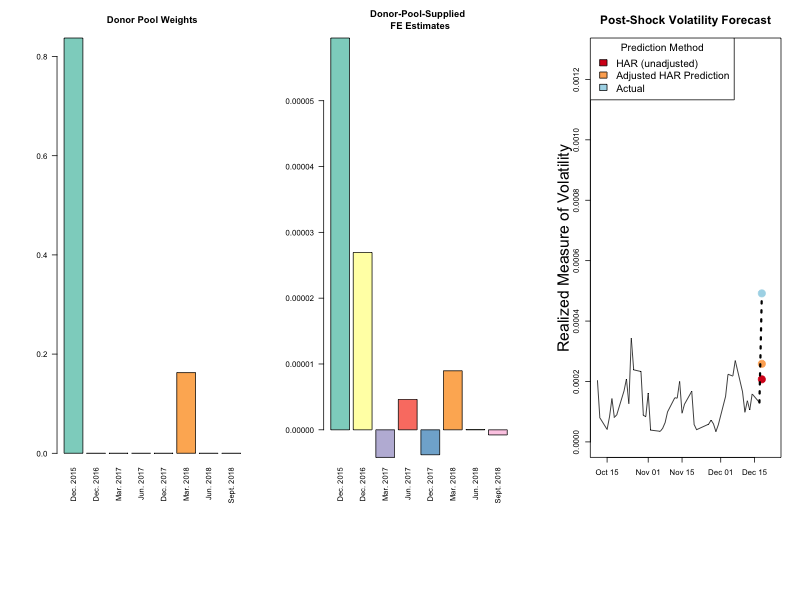
\includegraphics[scale=.4]{real_data_output_plots/savetime_SatJun151644072024__^VIX-^IRX-^XAU_^VIX_2018-12-18-2015-12-15-2016-12-13-2017-03-14-2017-06-13-2017-12-12-2018-03-20-2018-06-12-2018-09-25.png}
    \caption{Over the course of the 2010s, the US FOMC began a rate-hiking cycle.  Left pane: weights of the donor pool of FOMC meetings; right-pane: fixed effect estimates; right pane: the unadjusted forecast, adjusted forecast, and actual forecast}
    \label{fig:six_plots}
    \end{center}
  \end{figure}

\subsection{VAR}
Many time series, especially macroeconomic time series, naturally arise as constituents of groups of dependent variables that interact across time.
\subsection{LSTM/GRU}

Here we demonstrate the tremendous capaciousness of SPC by applying it to predictions generated by a pair of non-parametric forecasting functions, Long Short Term Memory and GRU.  We will re-examine an application found in \cite{lin2021minimizing}.

We borrow code from \cite{Brownlee_2022}

\begin{itemize}
  % \item \href{https://www.r-bloggers.com/2021/04/lstm-network-in-r/#google_vignette}{a}
  % \item \href{https://sharmasaravanan.medium.com/an-implementation-guide-for-lstm-in-r-2347e4118a2c}{b}
  % \item \href{https://search.r-project.org/CRAN/refmans/TSdeeplearning/html/GRU_ts.html}{c}
  % \item \href{https://medium.com/codex/time-series-prediction-using-lstm-in-python-19b1187f580f#:~:text=In%20conclusion%2C%20LSTM%20models%20are,in%20your%20data%20science%20toolkit.}{d}
  \item \href{https://machinelearningmastery.com/time-series-prediction-lstm-recurrent-neural-networks-python-keras/}{LSTM in Python}
\end{itemize}

\subsection{``Exponential Breaks"}
In \cite{castle2011forecasting}, the authors discuss intercept shifts that decay deterministically.  Those shifts are parameterized by a scalar $\lambda$ and a decay rate $\psi$.  We adapt their model for our own purposes:

\begin{align}
y_{i,t} = \alpha_{i} + \lambda[1 - e^{-\psi[t-T_{i}^{*}+1]}]\textbf{1}_{t\geq T_{i}^{*}+1} + \epsilon_{i,t}, \epsilon_{i,t} \simiid [0,\sigma^{2}] \text{ .}\label{decay_model}
\end{align}
This poses a novel case for our method, in that the model is parametric and yet without estimability of all shock parameters, aggregation may not be straightforward or easy.  Consider, for any $i$, $2 \leq i \leq n+1$, the estimates $\hat\alpha_{i,OLS}$  obtained via regression on the first $T_{i}^{*}+1$ points as well as $\hat\lambda_{OLS}$ obtained by estimating a fixed effect at $t=T_{i}^{*}+1$.  Consider also a subsequent estimator, an estimator for $\psi$, that is derivable from inverting the model specification and plugging-in the estimates  $\hat\alpha_{i,OLS},\hat\lambda_{OLS}$:

\begin{align}
\hat\psi_{i,plugin} = \frac{1}{T_{i}-(T_{i}^{*}+2)}\sum^{T_{i}}_{t\geq T_{i}^{*}+2}-log{\big[-\big(\frac{y_{i,t}-\hat\alpha_{i}}{\hat\lambda} -1\big)\big]} / [t-T_{i}^{*}+1]\text{ .}\label{plugin}
\end{align}
(\ref{plugin}) is, to put it lightly, a complicated estimator with potentially dubious properties.  To begin, (\ref{plugin}) is defined only when the term inside the logarithm is positive for each $t\geq T^{*}_{i}+2$.  We could get around this by dropping any summands for which that term is nonpositive and instead calculate an average over only the remaining subset of summands.  Variance estimates for $\hat\psi_{i,plugin}$ may require resampling methods or the delta method. 

Now consider a practitioner in need of a conditional forecast for $T_{1}^{*}+h, h\geq 1$.  Could aggregating the prediction residuals $r_{i,T_{i}^{*}+h} = y_{T_{i}^{*}+h}-\hat y_{i, T_{i}^{*}+h}, h\geq 1$ lead us to a superior predictions in the time series under study?\\

\textbf{Consider also these complicating scenarios}
\begin{enumerate}
  \item We can estimate $\lambda$ using a cross-sectional regression, and that may be better estimator than doing it one-by-one in each donor.
  \item Here we have taken $\lambda$ to be fixed and shared across donors.  If $\lambda$ is a function of a random effect, however, then estimating it becomes harder.
\end{enumerate}

\subsection{The Method of Multiple Shocks, Dual Shocks, and Shock-Partitioning}

Sometimes, we might have reason to believe that a forecast requires adjustment due to not one but multiple shocks.  \cite{lin2021minimizing} explored a ``dual'' shock in their analysis of oil company equity price shocks due to the March 2020 COVID lockdowns.  \\

Method 1: for each source of the $k$ shocks, assemble $n_{j}$ donors and $p_{j}$ covariates, with $j=2,...,n_{j}+1$, compute weights $\{\pi_{i,j}\}^{n_{j}+1}_{i=2}$.  With these $k$ weight sets, a set of $k$ aggregated shock estimators can be constructed and averaged (or aggregated in some other way).

Method 2: the $k$ shocks can be represented using one application of distance-based weighting, with the vector $\delta$ and the vector $\x_{i,T^{*}_{i}+1}$ can encode a partition of shocks by using zeros in appropriate entries.

\section{Discussion}

The forecast horizon --- does it matter?  If so, how so?  \cite{lin2021minimizing} has a one-period horizon.  \cite{clements1998forecasting}{p. 203} discuss how long to keep the forecast adjustment in place.  For a corrected ``slope parameter'', the effect of $h$ is not so clear.\\

\subsection{Shock propagation and estimation accuracy}
Consider \cite{lundquist2024volatility}, in which a real world example shows how volatility can be forecasted following surprising election outcomes.  There, the estimation of fixed effects is done around elections in a donor pool.  That means that for each past election or poll, etcetera, the method must accurately estimate the surprise-induced volatility boost.  That means picking a window around such an effect.\\

\textbf{proposals}
\begin{enumerate}
  \item For a given data-generating process, simulate the accuracy and variability of shock estimates using post-shock measurement periods of difference lengths.
  \item Develop formal results to quantify (estimate, bound, etc) the risk of using different post-estimation measurement lengths.  This matters because it might be that a donor has experienced a shock in the last $m$ days, and if $m$ is too small, using that donor may be risky.
\end{enumerate}
    

\subsection{Aggregating residuals as opposed to aggregating fixed effect estimates?}

Cases:
\begin{enumerate}
  \item Fixed effect is estimated with accuracy 
  \item Fixed effect is estimated with considerable noise.  Hence, the idiosyncratic error is estimated with considerable noise.
  \item idiosyncratic error large
  \item idiosyncratic error small
\end{enumerate}  

\section{Extensions}\label{Extensions}

\begin{itemize}
  \item Forecast for series besides the mean or conditional mean \textcolor{red}{If you have a family of models estimated used a Gaussian loss function, and the post-shock residuals are not conditionally Gaussian (e.g. they could be conditionally Cauchy), then why even start with the default forecasting function?  Why not throw it out entirely?  If only the distribution of the innovations changes, then would that even matter for a forecast that is purely concerned with the conditional mean?}
  \item Bias-variance decomposition for ARIMA, as introduced in \ref{ARIMA} 
  \item Shrinkage estimation of autoregressive structure on all donors, then use our method
  \item TAR
  \item SETAR
  \item Function forecasts
  \item Binary Outcome Forecasts
  \item Density Forecasts
  \item Quantile Forecasts
\end{itemize}

\subsection{Forecast Combination}
what we are talking about here is not forecast combination, but there may be, nevertheless, a role for forecast combination: combining the forecasts generated by small differences in covariate and/or donor choice, as is done in \cite{lundquist2024volatility}. \\

Consider the leave-one-out method used on pairs of donors and covariates in \cite{lundquist2024volatility}.  By averaging over $(n+1)\cdot (p+1)$ predictions, we average over $n+1 \cdot p + 1$ convex combinations (where, when a donor is ommitted, its weight can be imputed as zero).

\subsection{Limitations}\label{Limitations}

\subsubsection{How important is a shared DGP?}
In particular, can we relax this assumption and proceed with weaker assumptions on the donors and time series under study?

\subsubsection{The assumption of a shared family can be relaxed in certain circumstances.  For example, if a certain donor is not like the time series under study with respect to the covariates, then the lack of a shared family will not matter much.}


\textbf{In Scope}
\begin{itemize}
  \item Introduce an existing diffuse set of approaches to adjusting forecasts (\ref{Introduction})
  \item Explain when/how similarity can help us forecast. \ref{outside_info}
  \item distinguish the method from various tools that inspired it (\ref{Introduction})
  \item show a few special cases, both examples and formal results (\ref{special_cases})
  \item discuss limitations of the method (\ref{Limitations})
  \item propose extensions (\ref{Extensions})
\end{itemize}
\textbf{Beyond Scope (but mentioned briefly)}
\begin{itemize}
  \item Wade too deeply into distance-based weighting details.  State that it's simply one way to do it.  Allude to \cite{lin2021minimizing,lundquist2024volatility}.
  \item wade too deeply into any of the special cases
  \item Tackle non-scalar random quantities (density forecasts, etc)
  \item Forecast combination
\end{itemize}

\clearpage

\bibliographystyle{plainnat}
\bibliography{unifying.bib}
 
\end{document}